
The results are presented in figure \ref{fig:alignment} and tables \ref{tab:subset_data}, \ref{tab:alignment} and \ref{tab:full_data}. 

Due to very high computational costs for some of the algorithms, both in time and memory, we were  not able to average over ten iterations as Lohdi et al. did for every entry in the tables. \textbf{Where this was most of an issue... }
We have clearly stated in the tables how many iterations were performed for that data. 
\begin{table}
	\centering
	\subfloat[NGK performance for different subequence lengths $ n $.]{
	\begin{tabular}{| c | c | c | c | c | } \hline
		NGK & $ n $ & Precision & Recall & $ F_1 $   \\ \hline	
		& 3 & 0.96 & 0.88 & 0.92     \\ 
		acq & 4 & 0.90 & 0.89 &  0.89    \\
		& 5 & 0.97 & 0.86 & 0.92     \\ \hline
		& 3 & 0.97 & 0.93 &  0.95    \\ 
		earn & 4 & 0.99 & 0.93 &  0.96    \\ 
		& 5 & 0.99 & 0.89 &  0.93    \\ \hline
		& 3 & 1 & 0.87 & 0.93     \\ 
		corn & 4 & 1 & 0.64 & 0.78     \\ 
		& 5 & 1 & 0.44 &  0.61    \\ \hline
		& 3 & 0.90 & 0.90 &  0.90    \\ 
		crude & 4 & 0.92 & 0.86 & 0.89     \\ 
		& 5 & 1 & 0.73 &  0.84    \\ \hline
	\end{tabular}
	}
\quad
	\subfloat[SSK performance for different sequence lengths $ n $. $ \lambda = 0.5 $ throughout.]{\begin{tabular}{| c | c | c | c | c | }\hline
			SSK & $ n $ & Precision & Recall & $ F_1 $   \\ \hline	
			& 3 & 0.93 & 0.96 & 0.94     \\ 
			acq& 4 & 0.93 & 0.96 &  0.94  \\
			& 5 & 0.97 & 0.93 & 0.95    \\ \hline
			& 3 & 0.99 & 0.93 & 0.96  \\ 
			earn& 4 & 0.99 & 0.95 &  0.97   \\
			& 5 & 0.99 & 0.96 & 0.97    \\  \hline
			& 3 & 0.97 & 0.87 & 0.91  \\ 
			corn& 4 & 0.98 & 0.64 & 0.88    \\ 
			& 5 & 0.98 & 0.44 &  0.83    \\ \hline
			& 3 & 0.97 & 0.86 &  0.88   \\ 
			crude& 4 & 0.98 & 0.80 & 0.91   \\ 
			& 5 & 0.98 & 0.73 &  0.88  \\ \hline
	\end{tabular} }

	\subfloat[WK performance results, averaged over 10 iterations. Numbers in parenthesis are reference value from Lodhi et al.]{
	\begin{tabular}{| c | c | c | c | } \hline
		WK  & Precision & Recall & $ F_1 $   \\ \hline	
		acq &  0.974  & 0.930  & 0.951 (0.802) \\ \hline
		earn &   0.978 & 0.972 & 0.976 (0.925)  \\ \hline
		corn &   0.992  & 0.867  &  0.923 (0.762) \\ \hline
		crude &   0.946  & 0.957  &  0.948 (0.904) \\ \hline	
	\end{tabular}}

	\subfloat[SSK performance results with varying $ \lambda $ . $ n=5 $ throughout.]{\begin{tabular}{| c | c | c | c | c | } \hline
			SSK & $ \lambda  $& Precision & Recall & $ F_1 $   \\ \hline	
			& 0.05 & 1 & 0.92 & 0.96     \\ 
			acq & 0.1 & 1& 1 &  1    \\
			& 0.5 & 0.89 & 1 & 0.94     \\ \hline
			& 0.05 & 1 & 0.98 &  0.99    \\ 
			earn & 0.1 & 0.98 & 1 &  0.99    \\ 
			& 0.5 & 1 & 0.90 &  0.95    \\ \hline
			& 0.05 & 1 & 0.87 & 0.93     \\ 
			corn & 0.1 & 1 & 0.87 & 0.93     \\ 
			& 0.5 & 0.94 & 1 &  0.97   \\ \hline
			& 0.05 & 0.90 & 0.75 &  0.82    \\ 
			crude & 0.1 & 1 & 0.91 & 0.95     \\ 
			& 0.5 & 1 & 0.70 &  0.82    \\ \hline
	\end{tabular}}
\caption{Results from SSK, NGK and WK using subset of Reuters dataset.\label{tab:subset_data}}
\end{table}


\begin{figure}
	\centering
	\subfloat[Our results]{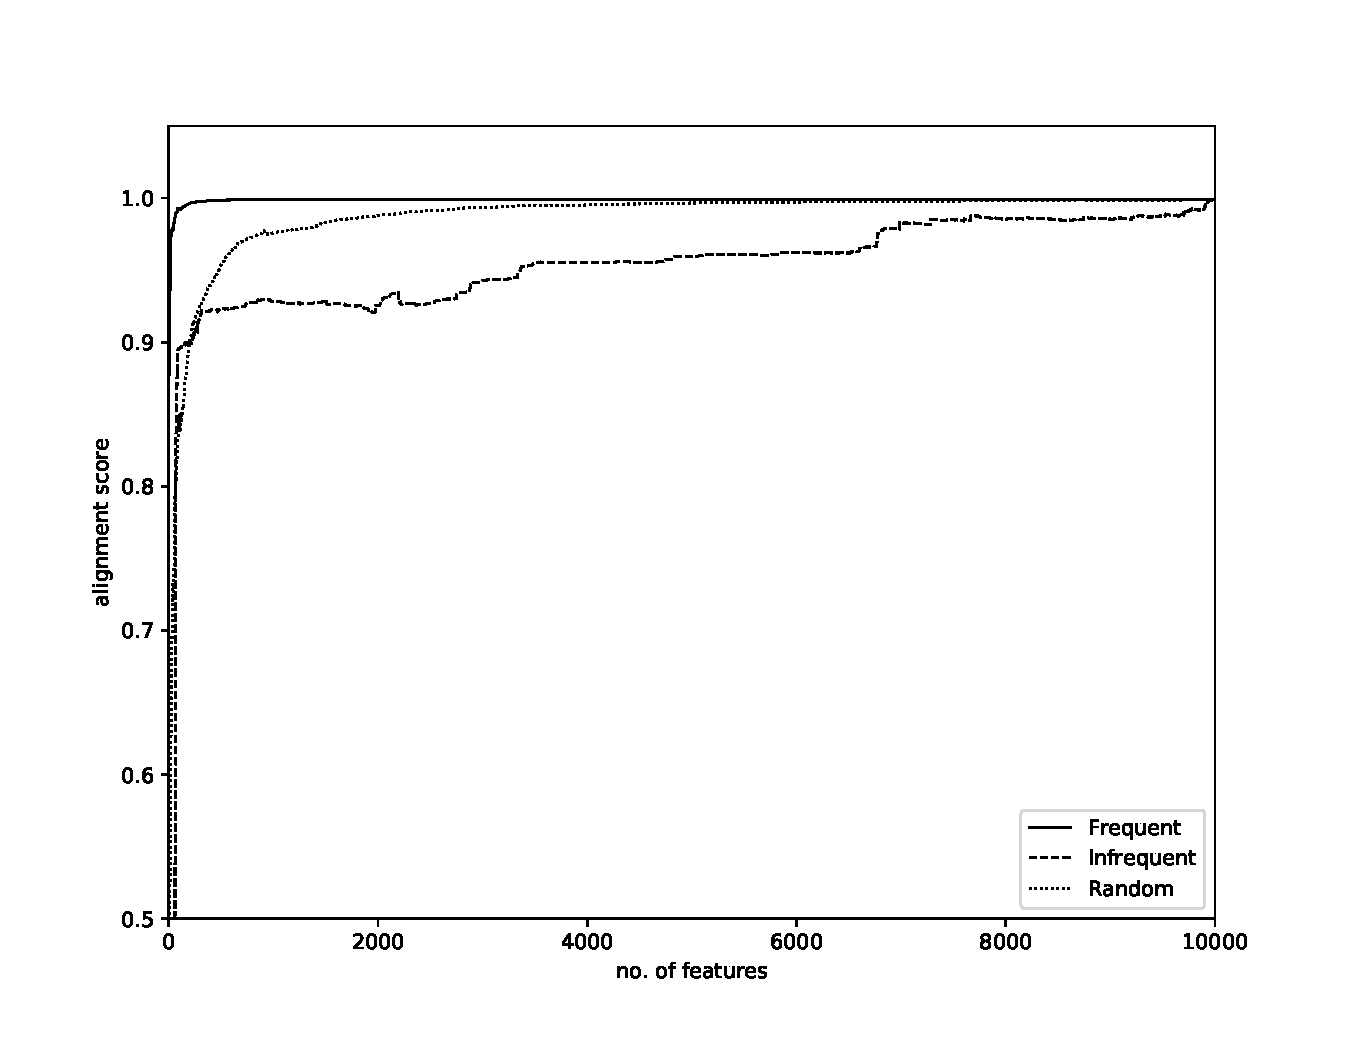
\includegraphics[height = 6.25cm]{../plots/Alignment_scores.pdf}}
	\subfloat[Lohdi et al.'s]{\raisebox{0.57cm}%
		{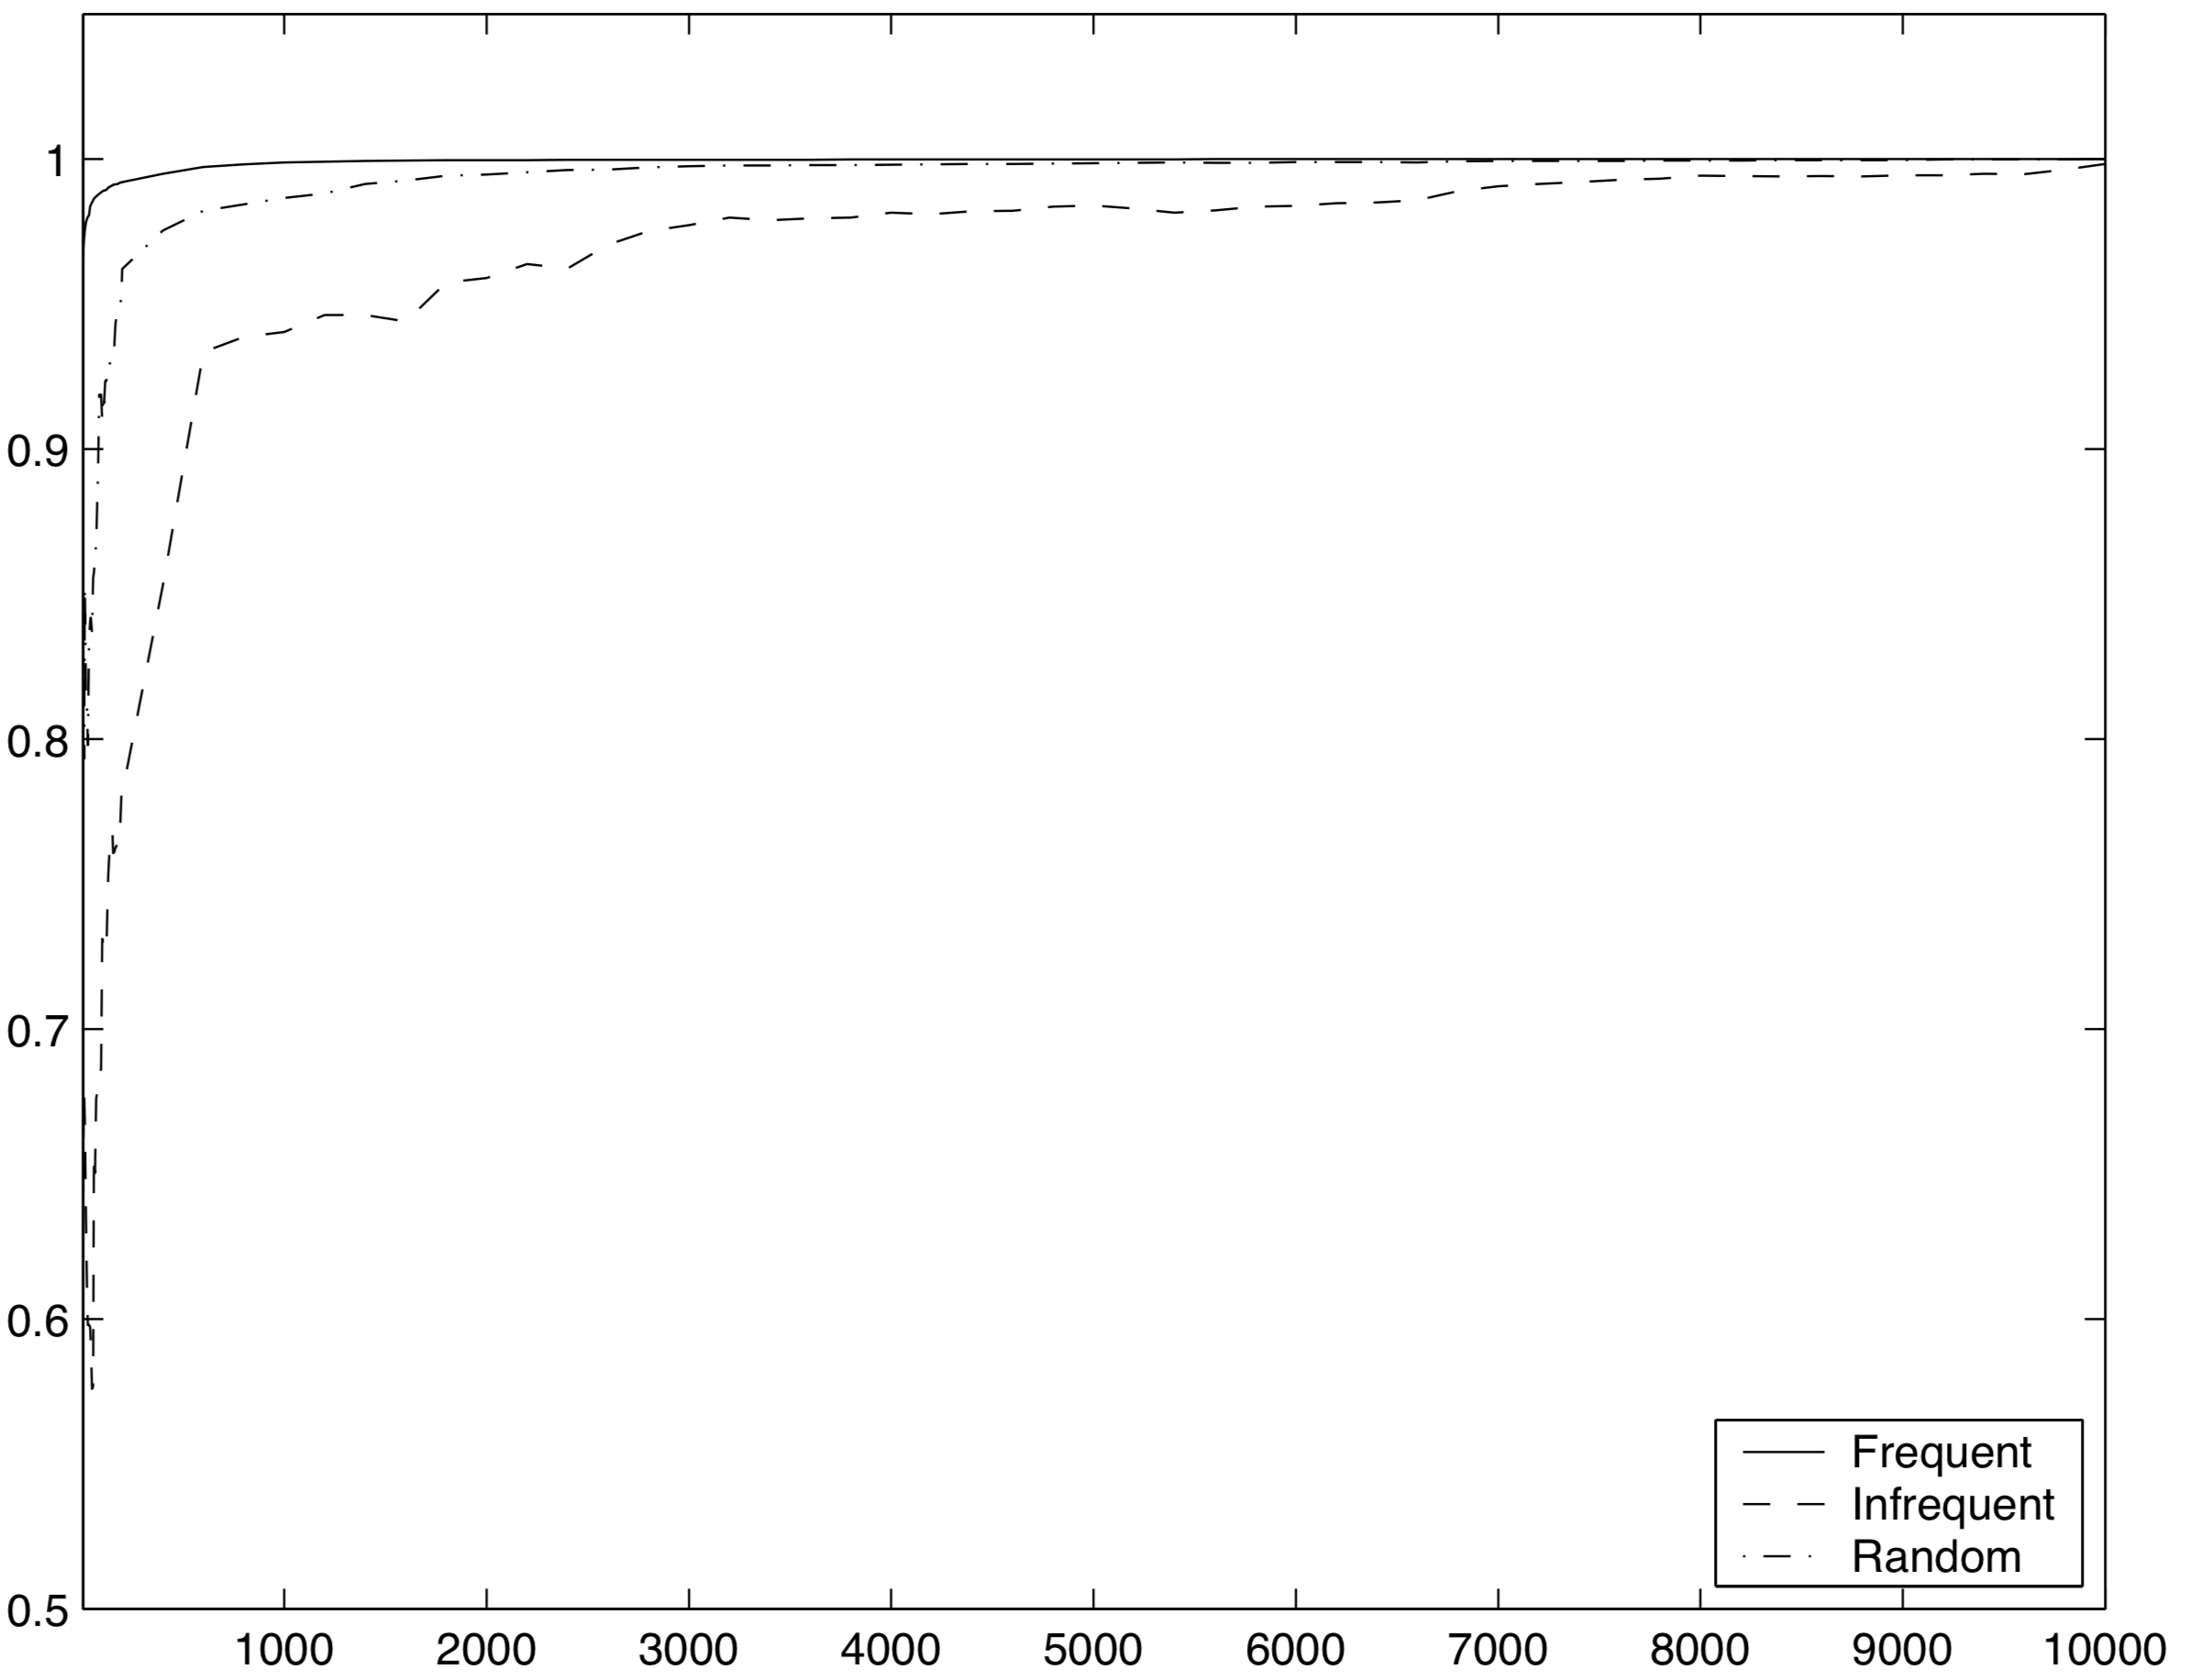
\includegraphics[height = 5cm]{../plots/Lodhi_alignment_score.png}}}%
	\caption{Alignment scores for varying the number of vectors $ x $ in the subset $ \tilde{S} $. Lohdi et al.'s figure is shown for comparison.\label{fig:alignment}}
\end{figure}

\begin{table}
	\centering
	\begin{tabular}{| c | c | c | }\hline
		aSSK & $ x $ = 1000 & $ x $ = 3000   \\ \hline
		acq & 0.96 (0.88)& 0.97 (0.85)\\ \hline
		earn & 0.98 (0.97) & 0.98  (0.97) \\ \hline
		ship & 0.43 (0.10) & 0.63  (0.53) \\ \hline
		corn & 0.84 (0.15) & 0.89 (0.65) \\ \hline
	\end{tabular} 
	\caption{F1 performance of the approximative SSK using 1000 and 3000 vectors in $ \tilde{S} $. $ n = 5 $ and $ \lambda = 0.5 $. Lodhi's results in parenthesis for comparison.\label{tab:alignment}}
\end{table}


\begin{table}
	\centering	
	\begin{tabular}{| c | c | c | c | c | c | c | c |}\hline
		& WK & NGK & NGK  & NGK  & aSSK & aSSK& aSSK \\ 
		&  & $n = 3$& $ n = 4 $ & $ n = 5 $ & $ n = 3 $& $ n = 4 $ & $ n = 5 $ \\ \hline
		earn & 0.98 & 0.98 &  0.98&  0.98 & 0.98 & 0.98 & 0.98 \\ \hline
		acq & 0.97 & 0.95 &  0.95 &  0.96 & 0.95 & 0.95 & 0.95 \\ \hline
		money-fx & 0.79 & 0.77 &  0.79 & 0.77 & 0.77 & 0.8 & 0.78 \\ \hline
		grain & 0.92 & 0.81 &  0.83& 0.82 & 0.84 & 0.86 & 0.8 \\ \hline
		crude & 0.87 & 0.84 &  0.85 & 0.8 & 0.82 & 0.79 & 0.73 \\ \hline
		trade & 0.8 & 0.73 &  0.77 & 0.77 & 0.72 & 0.79 & 0.77 \\ \hline
		interest & 0.8 & 0.72 &  0.73 & 0.75 & 0.79 & 0.8 & 0.77 \\ \hline
		ship & 0.78 & 0.66 &  0.55 & 0.47 & 0.69 & 0.5 & 0.34 \\ \hline
		wheat & 0.79 & 0.86 &  0.84 & 0.8 & 0.8 & 0.8 & 0.76 \\ \hline
		corn & 0.86 & 0.73 &  0.85 & 0.65 & 0.78 & 0.72 & 0.6 \\ \hline	
	\end{tabular}
\caption{Lodhi et al.'s ten best performing classes with our $ F_1 $ results for WK, NGK and  aSSK using the entire Reuters dataset. For aSSK; $ \lambda = 0.5 $\label{tab:full_data} }
\end{table}


\subsection{Eriks kommentarer}
\begin{itemize}
	\item We can clearly see that NGK performs well for small N, but considerably worse for larger N (see appendix)
	
	\item Like it's algorithmic cousin the NGK, it performs well for relative small k, but less well for larger k (again, see appendix for all data)
	
	\item  Varying $ \lambda $ shows that SSK is not that sensitive to values of $ \lambda $. Generally we can see that unless you choose more extreme values, the SSK performs well.
	
	\item Lodhi's results in parenthesis. This allows us to verify our implementation of the approximation kernel, but is not used for extensive results analysis.
\end{itemize}
